% Template for ICIP-2018 paper; to be used with:
%          spconf.sty  - ICASSP/ICIP LaTeX style file, and
%          IEEEbib.bst - IEEE bibliography style file.
% --------------------------------------------------------------------------
\documentclass{article}
\usepackage{spconf,amsmath,graphicx}

\graphicspath{ {images/} }

% Example definitions.
% --------------------
\def\x{{\mathbf x}}
\def\L{{\cal L}}

% Title.
% ------
\title{Fine Tuning The Rotating Skip List}
%
% Single address.
% ---------------
\name{Itamar Talmon, Tal Shoef}
\address{Tel Aviv University}

\begin{document}
%\ninept
%
\maketitle
%
\begin{abstract}
Skip list \cite{C3} is a linked-list-based structure that became an increasingly popular concurrent alternative to search trees due to its logerithmic complexity and local balancing operation. The Rotating skip list \cite{C1} is the fastest concurrent skip list to date. In this paper, we investigate, and try to improve upon, the different heuristics used in the Rotating skip list data structure.
\end{abstract}
%
\section{Introduction}
\label{sec:intro}

\subsection{Concurrent Skip Lists}
\label{ssec:csl}
Skip lists are probabilistic search structures which provide improved execution time bounds compared with straightforward binary search trees yet are much simpler to implement than any guaranteed-$O(\log{n})$ search structure \cite{C3}.
A skip list comprises multiple levels, each of which is a linked list. Every skip-list node is present at the lowest level, and probabilistically present in each higher level up to some maximum level that is chosen independently and randomly for each node. This maximum is selected using a random number generator with
exponential bias: for example, the probability of inserting into level $x$ is often chosen to be $2^{-x}$.
Due to its logerithmic complexity, simplicity and local balancing operation, skip list became an increasingly popular concurrent alternative to search trees and  the default JDK logarithmic concurrent structures (which is an implementation of the lock-free skip list algorithm suggested by Fraser\cite{C4}). Another particularly useful property for parallel skip-list design is that a node can be independently inserted at each level in the list. A node is visible as long as it is linked into the lowest level of the list: insertion at higher levels is necessary only to maintain the property that search time is $O(\log{n})$. This lead to an improved algorithm \cite{C2} that avoids contention hotspots by relying on a maintenance thread to raise, lower and clean-up the towers. This technique lets application threads simply insert an element at the bottom or delete an element by marking it as logically deleted. Yet, untill recently, typical skip list did not exploit multicore platforms as well as trees. This has changed when the Rotating skip list was introduced. The Rotating skip list \cite{C1} combines the rotation of trees and the uncontended nature of skip lists into a multicore-friendly data structure. The core algorithmic novelty is the use of wheels instead of the usual towers that are linked together to speedup traversals.

\subsection{Rotating Skip List Algorithm}
\label{ssec:trsl}

In this section, we present an overview of the rotating skip list key-value store implementation. The rotating skip list differs from traditional skip lists in that it is deterministic and uses wheels, its rotations differ from trees rotations in that they execute in constant time to lower the structure. The resulting algorithm is proven to be linearizable and non-blocking (or lock-free). Refer to \cite{C1} for more details, figures, pseudo code and corectness proofs.

\subsubsection{Key-value store}
\label{ssec:ksv}

Key-value stores offer the basis for indexes to speed up access to data sets. They support the following operations:
\begin{itemize}
	\item  $put(k,v)$ inserts the key-value pair $<k, v>$ and returns $true$ if $k$ is absent, otherwise return $\bot$
	\item  $delete(k)$ removes $k$ and its associated value and returns $true$ if $k$ is present in the store, otherwise return $false$ 
	\item  $get(k)$ returns the value associated with key $k$ if $k$ is present in the store, otherwise return $false$
\end{itemize}

\subsubsection{Structure Memory}
\label{ssec:sm}

Locality is achieved by using a rotating array sub-structure, called the wheel, detailed later in a separate section. The structure is a skip list, denoted $sl$, specified with a set of nodes, including two sentinel nodes. The head node is used as an entry point for all accesses to the data structure, it stores a dummy key that is the lowest of all possible keys. A tail node is used to indicate the end of the data structure, its dummy key is strictly larger than any other possible keys. As in other skip lists, node values are ordered in increasing key order from left to right. The global counter ZERO indicates the index of the first level in the wheels, it is set to 0 intially. The node structure contains multiple fields. It first contains a key-value pair denoted by $<k, v>$. Two special values $v = \bot$ and $v = node$ indicate that the node is logically deleted and physically deleted, respectively. A node is first logically deleted before being physically removed and two logically deleted nodes cannot share the same key $k$. The level represents the level of this node’s wheel, similar to the level of the corresponding tower in a traditional skip list, it indicates that the node keeps track of successors indexed from 0 to level − 1. The succs is the node’s wheel, it stores the successor pointer at each level of the node. next (resp. prev) is a direct pointer to the next (resp. previous) node that contains the smallest key larger than $k$ (resp. the highest key lower than $k$). Hence the skip list nodes are all linked through a doubly linked list. This doubly linked list allows to backtrack among preceding nodes if the traversal ends up at a deleted node. Finally, the marker is a special mark used only during physical removal. 

\subsubsection{Traversal}
\label{ssec:trv}

Each update operation ($put$, $delete$) avoids contention hotspots by localizing the modification to the least contended part of the data structure. All adjustments to the upper levels are sequentially executed by a dedicated maintenance thread, described later, hence allowing a deterministic adjustment of the levels. Any traversal, whether it is for updating or simply searching the structure, is executed from the top of the head node traversing wheels from left to right and levels from top to bottom. Each access looks for the position of some key $k$ in the skip list by starting from the top level of the head down to the bottom level. The $get$ function starts by traversing the structure from the skip list head, namely $sl.head$, till the bottom level. It records the value of ZERO at the beginning of the traversal into a local zero variable, sets its starting point to the $set.head$ before iterating over each level $i$ from the top level of the skip list, which is also the top level of the head $set.head.level - 1$, to zero. Once the $get$ has reached the bottom level, $node$ is actually set to the node with the largest key $k^{'}< k$. If this node is physically deleted, the traversal backtracks among deleted nodes and invokes $help remove$ to notify the background thread of the nodes to be removed. Note that the traversal can thus reach a node that is not linked by any succs pointer but only one next pointer. Then it updates $next$ to the immediate next node ($node.next$). Once the right position at the bottom level indicated by $next.k > k$ is reached, the targeted key $k$ is checked. If it is non logically deleted, the associated value $val$ is returned, otherwise $\bot$ is  returned to indicate that no key $k$ was present in the key-value store. The $put$ function is similar in that it first traverses the structure from top to bottom, backtracks from right to left and help remove deleted nodes. The $put$ may find that the node with the key it looks for is logically deleted, in which case it simply needs to logically insert it by setting its value to the appropriate one using a CAS. if the node is found as non logically deleted, then put is unsuccessful and returns $false$. Finally, if the put did not find the targeted key $k$, it creates a new node node with key $k$ and value $v$ that is linked to next and inserts it physically using a CAS . The reason why nodes are logically deleted before being physically removed is to minimize contention. The delete function marks a node as logically deleted by setting its value to $\bot$. A separate maintenance thread is responsible for traversing the bottom level of the skip list to clean up the deleted nodes as described in later section. The delete executes like the $put$ as it also traverses the structure from top to bottom and backtracks to help remove the deleted nodes. It checks whether a key is absent or if its node is logically or physically deleted in which case it returns $false$. Otherwise, this function logically deletes the node using a CAS to mark it. \textbf{A heuristic helps deciding whether the delete should help removing. This happens only when the ratio of logically deleted nodes over non-logically deleted nodes (as communicated by the background thread) reaches 3 after what it pays off}. Whether it helps physically removing or not, the delete returns $true$ if the node was logically deleted.

\subsubsection{Wheels instead of towers}
\label{ssec:wiot}

The wheel size is adjusted without having to mutate a pointer, simply by over provisioning a static array and using modulo arithmetic to adjust the mutable levels. The modulo arithmetic guarantees that increasing the index past the end of an array wraps around to the beginning of the array. This allows lowering to be done in constant-time by simply increasing the index of the lowest logical level of all the arrays without incurring contention. A global variable ZERO is used to keep track of the current lowest level, and when a lowering occurs the lowest index level is invalidated by incrementing the ZERO variable. This causes other threads to stop traversing the index levels before they reach the previous lowest level of pointers. If ZERO is increased above the length of the array this will not compromise the program since the arrays are accessed with modulo arithmetic. To illustrate how wheels improve locality of reference, consider testing to see if the current node next in the traversal has a key greater than the search key. If the wheels were represented using distinct objects, then $next.k$ would need to be changed to $next.node.k$, reflecting the fact that the key-value information is being stored in a distinct node object from the index next references. This extra layer of indirection can hurt performance of the skip list, especially since this redirects all traversals.

\subsubsection{Background thread}
\label{ssec:bt}

The background (or maintenance) thread executes a loop where it sleeps for 50 microseconds (\textbf{a heuristic parameter}). The maintenance thread raises wheels of non-deleted nodes by calling the $raise bottom level$ function. This raise is compensated with a constant-time lowering specific to the algorithm. This periodic adaptation makes it unnecessary to use the traditional pseudo-random generators as the lowering and raising (the action of increasing the height of a tower) become deterministic. The $lower skiplist$ function discards, in constant-time, the entire bottom level of the skip list by simply changing the ZERO counter used in the modulo arithmetic, without blocking application threads. Note that the $lower skiplist$ is followed by a $cleanup bottom$ level that takes linear time to reclaim the memory of the deleted level, however, all traversals starting after the ZERO increment ignores this level. The $lower skiplist$ function is called, with some heuristic, only if is lowering necessary returns true. \textbf{The chosen heuristic was if there are 10 times more deleted nodes with height greater than 1 than bottom-level nodes}. The $raise bottom level$ also cleans up the skip list by removing the logically deleted nodes. After all logically deleted nodes are discarded, their wheels having been progressively lowered down to a single level, they are garbage collected using an epoch based memory reclamation algorithm discussed later on. The $raise node$ and $raise index level$ simply consist, for each level from bottom to top, of raising each node in the middle of three consecutive non-deleted nodes of the same height. The $help remove$ function called by the $remove$ function or by an application thread removes the deleted nodes. It actually only removes nodes that do not have any wheel successors. Nodes with wheels are removed differently by first lowering their levels. Deleted wheels are simply removed later by the background thread within a $help remove$ during maintenance. Note that at the end of the removal the prev field can be updated without synchronization as it does not have to be set to the immediate previous node.

\subsubsection{Memory reclamation}
\label{ssec:bt}

The memory reclamation of our rotating skip list is based on an epoch based garbage collection algorithm similar to the one used in Fraser’s skip list \cite{C4} with some differences. The garbage collector of Fraser’s skip list is partitioned into sections responsible for managing nodes of a particular skip list level. Partitioning the memory manager like this means that requests to the memory manager regarding different skip list levels do not need to conflict with one another. In contrast, the rotating skip list does no such partitioning of memory management responsibilities, since the rotating skip list uses only one node size for all list elements regardless of their level. This increases the probability of contention in the memory reclamation module when a large number of threads issue memory requests simultaneously.


\subsection{Our Contribution}
\label{ssec:oc}

We examined and extended the following heuristics:

\begin{itemize}
	\item Level Hight Heuristics
	\item Level Delete Heuristics 
	\item Deletion Help Heuristics
	\item Background Thread Sleeping Heuristics 
\end{itemize}

\hfill \break
Detailed descriptions of the changes made, in addition to the evaluations, are included in the prociding sections of the paper.

\subsection{Code Location}
\label{ssec:cl}
The complete code, including the compiled data strucures and the evaluation script, could be find at \\\texttt{github.com/itamartalmon/synchrobench}.

\section{LEVEL HIGHT HEURISTICS}
\label{sec:lhh}

The Maximum Level of the data structure , BLABLABLA

\subsection{Fixed Max Level}
\label{ssec:fml}

Fixing the Max level is commonly use, blablblal

As can be seen on figure BLABLALB, ads
bla bla bla bla bla bla
bla bla bla bla bla 
bla bla bla bla bla bla
bla bla bla bla bla 
bla bla bla bla bla bla
bla bla bla bla bla 
bla bla bla bla bla bla
bla bla bla bla bla bla
bla bla bla bla bla 
bla bla bla bla bla bla
bla bla bla bla bla 
bla bla bla bla bla bla
bla bla bla bla bla 
bla bla bla bla bla bla
bla bla bla bla bla bla
bla bla bla bla bla 
bla bla bla bla bla bla
bla bla bla bla bla 
bla bla bla bla bla bla
bla bla bla bla bla 
bla bla bla bla bla bla

\subsection{Dynamic Max Level}
\label{ssec:dml}

Dynamic Max level is more blablblal

\subsubsection{Evaluation}
\label{sssec:ml-evl}

As can be seen on figure bla bla bla bla bla 
bla bla bla bla bla bla
bla bla bla bla bla 
bla bla bla bla bla bla
bla bla bla bla bla 
bla bla bla bla bla bla
bla bla bla bla bla 
bla bla bla bla bla bla

\begin{figure}
	\caption{Max Level Heuristics Performence}
	\centering
	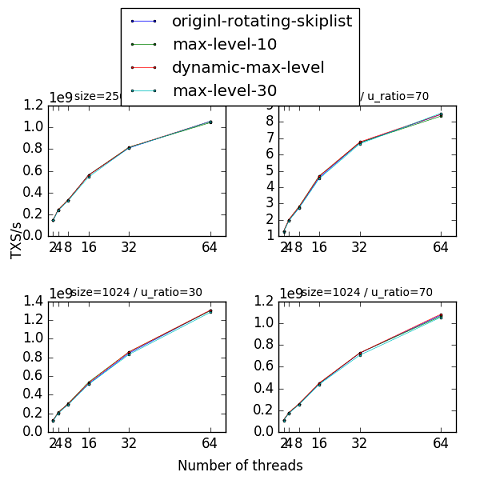
\includegraphics[width=0.4\textwidth]{max-level_plot}
\end{figure}

bli bla blu

\section{ROTAION DELETION HEURISTICS}
\label{sec:rdh}

When deleting blablabae , BLABLABLA

\subsection{Tall-Deletions-Size Rate}
\label{ssec:tds}

In the original paper use, blablblal

\subsubsection{Evaluation}
\label{sssec:tds-evl}

As can be seen on figure BLABLALB, ads
bla bla bla bla bla bla
bla bla bla bla bla 
bla bla bla bla bla bla
bla bla bla bla bla 
bla bla bla bla bla bla
bla bla bla bla bla 
bla bla bla bla bla bla
bla bla bla bla bla bla
bla bla bla bla bla 
bla bla bla bla bla bla
bla bla bla bla bla 
bla bla bla bla bla bla
bla bla bla bla bla 
bla bla bla bla bla bla

\begin{figure}
	\caption{Tall Delelted By Size Deletion Performence}
	\centering
	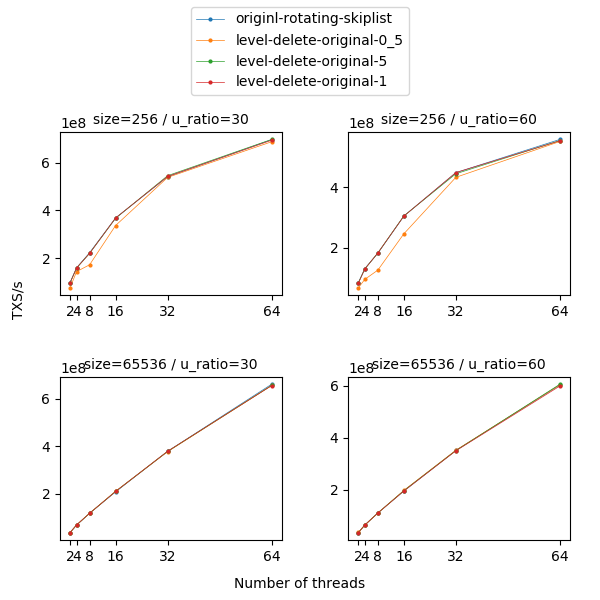
\includegraphics[width=0.4\textwidth]{level-delete-original_plot}
\end{figure}

\subsection{Relative Level Size}
\label{ssec:rls}

Dynamic Max level is more blablblal

\subsubsection{Evaluation}
\label{sssec:rls-evl}

As can be seen on figure BLABLALB, ads
bla bla bla bla bla bla
bla bla bla bla bla 
bla bla bla bla bla bla
bla bla bla bla bla 
bla bla bla bla bla bla
bla bla bla bla bla 
bla bla bla bla bla bla

\begin{figure}
	\caption{Levels Ratio Deletion Performence}
	\centering
	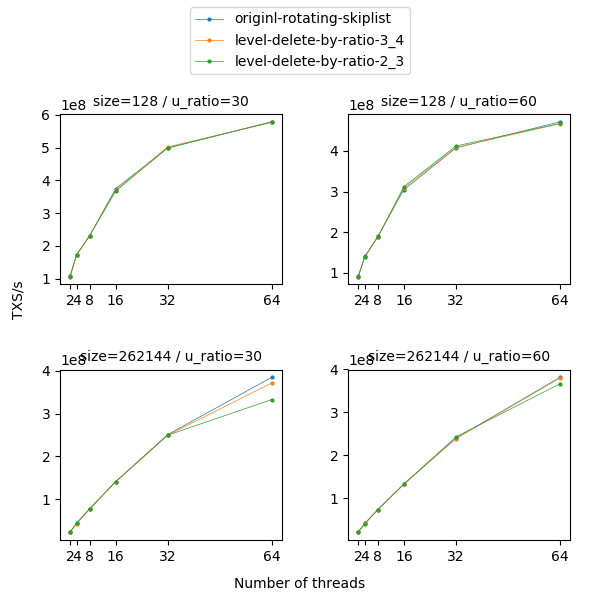
\includegraphics[width=0.4\textwidth]{level-delete-by-ratio_plot}
\end{figure}


\section{DELETION HELP HEURISTICS}
\label{sec:dhh}

\subsection{Thread-Num-Size Rate}
\label{ssec:tns}

Dynamic Max level is more blablblal

\subsubsection{Evaluation}
\label{sssec:tns-evl}

As can be seen on figure BLABLALB, ads
bla bla bla bla bla bla
bla bla bla bla bla 
bla bla bla bla bla bla
bla bla bla bla bla 
bla bla bla bla bla bla
bla bla bla bla bla 
bla bla bla bla bla bla

\begin{figure}
	\caption{Help-Remove Performence}
	\centering
	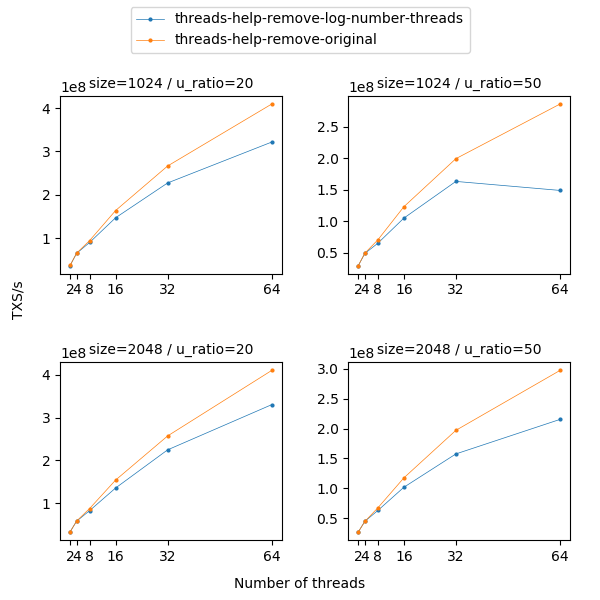
\includegraphics[width=0.4\textwidth]{help-remove_plot}
\end{figure}

\section{BACKGROUND THREAD SLEEP HEURISTICS}
\label{sec:bts}

The background blablabae , BLABLABLA

\subsection{Thread-Num Rate}
\label{ssec:dsrs}

In the original paper use, blablblal

\subsubsection{Evaluation}
\label{sssec:dsrs-evl}

As can be seen on figure BLABLALB, ads

\begin{figure}
	\caption{Background Sleep Time Performence}
	\centering
	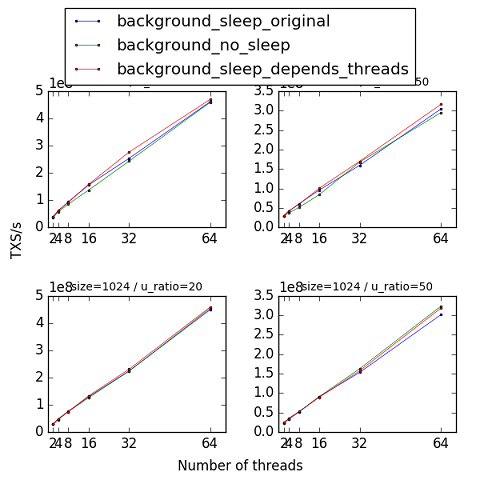
\includegraphics[width=0.4\textwidth]{sleep_plot}
\end{figure}


\section{Experimental Settings}
\label{sec:exp}

We used multicore machine with 8 AMD x86_64 Opteron(tm) Processor 6376 each have 8 cores that runs at 2.4 GHz. with L1d cache size of 16K, L1i cache size of 64K, L2 cache size of 2048K and L3 cache size of 6144K.

\section{Future Research}
\label{sec:foot}

BLIA BALIDSA ADBLADS


% To start a new column (but not a new page) and help balance the last-page
% column length use \vfill\pagebreak.
% -------------------------------------------------------------------------
%\vfill
%\pagebreak


% References should be produced using the bibtex program from suitable
% BiBTeX files (here: strings, refs, manuals). The IEEEbib.bst bibliography
% style file from IEEE produces unsorted bibliography list.
% -------------------------------------------------------------------------
\bibliographystyle{IEEEbib}
\bibliography{refs}

\end{document}
